\section{Six-system multi-arm endpoint perturbation campaign}
\label{sec:endpoint_perturbation_campaign}

We evaluated the response of six dopant--host systems, Cr/V/Mn embedded in
\ce{Sb2Te3} and \ce{Bi2Te3}, to three endpoint-relaxation arms: the historical
unperturbed endpoint (Base), a $+0.20$~\AA{} dopant displacement (Perturb A),
and a displacement of $(-0.10,+0.14,+0.10)$~\AA{} (Perturb B).  The campaign
contains 47 endpoint sites per system and arm, for 846 formal MACE relaxation
tasks.  All tasks passed the finite-value, topology, minimum-distance,
displacement, and scientific-success gates.  These results are model-relaxation
observables from Foundation-MACE with fixed-cell ASE FIRE relaxation; they are
not DFT, magnetic, or oxidation-state assignments.

\begin{table*}[t!]
\caption{\textbf{Measured multi-arm endpoint-relaxation summary.} Values are medians over the 47 historical endpoint sites for each of six host--dopant systems and each perturbation arm. ``Conv.'' reports the number of FIRE relaxations reaching $f_{\max}\leq0.03$ eV\,\AA$^{-1}$; $E_f$ is the final MACE energy, $F_{\max}$ the final maximum force, $d_{\max}$ the maximum atomic displacement from the perturbed input, and ``steps'' the FIRE step count. All 846 formal tasks passed the finite-value, topology, minimum-distance, displacement, and scientific-success gates. The Foundation-MACE model and fixed-cell FIRE protocol are the same across arms; this table reports model-relaxation observables, not DFT or magnetic conclusions.}
\label{tab:multiarms_endpoint_relaxation}
\centering\scriptsize
\setlength{\tabcolsep}{3.0pt}\renewcommand{\arraystretch}{1.08}
\resizebox{\textwidth}{!}{%
\begin{tabular}{@{}l*{12}{r}@{}}\toprule
 & \multicolumn{4}{c}{\textbf{Base}} & \multicolumn{4}{c}{\textbf{Perturb A: }$+x\,0.20$} & \multicolumn{4}{c}{\textbf{Perturb B: }$(-x,+y,+z)$} \\
\cmidrule(lr){2-5}\cmidrule(lr){6-9}\cmidrule(lr){10-13}
\textbf{System} & \textbf{Conv.} & $E_f$ & $F_{\max}$ & $d_{\max}$ & \textbf{Conv.} & $E_f$ & $F_{\max}$ & $d_{\max}$ & \textbf{Conv.} & $E_f$ & $F_{\max}$ & $d_{\max}$ \\
 & (47) & (eV) & (eV/\AA) & (\AA) & (47) & (eV) & (eV/\AA) & (\AA) & (47) & (eV) & (eV/\AA) & (\AA) \\ \midrule
Cr@Sb2Te3 & 47/47 & -299.679 & 0.027 & 0.024 & 47/47 & -299.690 & 0.028 & 0.196 & 47/47 & -299.696 & 0.026 & 0.192 \\
V@Sb2Te3 & 47/47 & -299.465 & 0.027 & 0.130 & 47/47 & -299.478 & 0.026 & 0.231 & 47/47 & -299.462 & 0.025 & 0.235 \\
Mn@Sb2Te3 & 47/47 & -299.344 & 0.027 & 0.132 & 47/47 & -299.343 & 0.028 & 0.227 & 47/47 & -299.343 & 0.027 & 0.231 \\
Cr@Bi2Te3 & 47/47 & -300.835 & 0.026 & 0.473 & 47/47 & -300.823 & 0.026 & 0.489 & 47/47 & -300.834 & 0.027 & 0.471 \\
V@Bi2Te3 & 47/47 & -300.594 & 0.026 & 0.495 & 47/47 & -300.609 & 0.026 & 0.527 & 47/47 & -300.581 & 0.026 & 0.551 \\
Mn@Bi2Te3 & 47/47 & -300.708 & 0.028 & 0.499 & 47/47 & -300.708 & 0.026 & 0.528 & 47/47 & -300.707 & 0.027 & 0.532 \\
\bottomrule\end{tabular}}
\vspace{2pt}
\parbox{0.98\textwidth}{\scriptsize \textit{Arm definitions.} Base is the unperturbed historical endpoint. Perturb A displaces the dopant by $(+0.20,0,0)$\,\AA; Perturb B uses $(-0.10,+0.14,+0.10)$\,\AA (norm $0.199$\,\AA). Medians summarize distributions and should not be read as endpoint-level equivalence.}
\end{table*}


\begin{figure}[p]
\centering
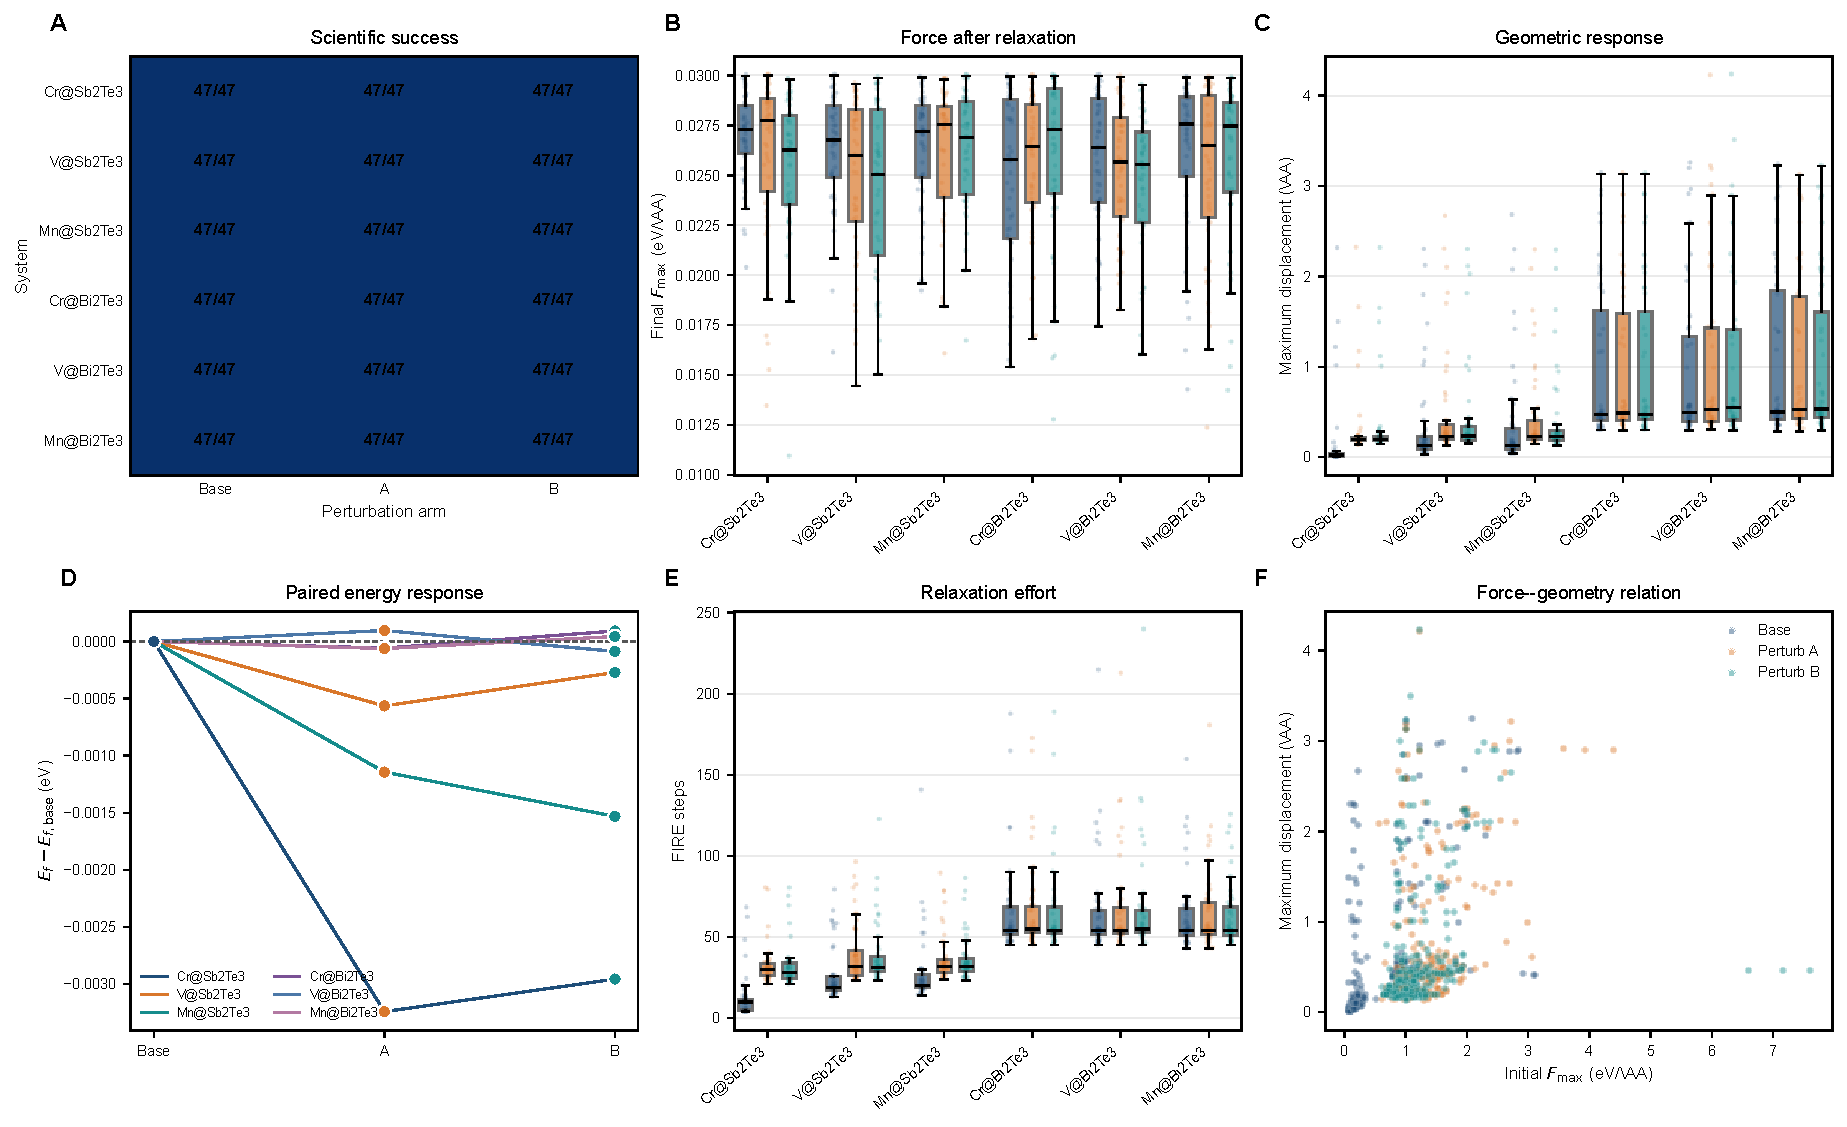
\includegraphics[width=\textwidth]{revision1/appendix/figures/fig1_campaign_overview.pdf}
\caption{\textbf{Campaign overview and relaxation outcomes.} (A) Scientific
success across all 846 formal tasks. (B--C) Final-force and maximum-displacement
distributions by perturbation arm. (D) Paired energy responses relative to the
Base arm. (E) FIRE-step distributions. (F) Initial force versus final
displacement. Points and distributions retain endpoint-level variation rather
than showing only system medians.}
\label{fig:endpoint_campaign_overview}
\end{figure}

\begin{figure}[p]
\centering
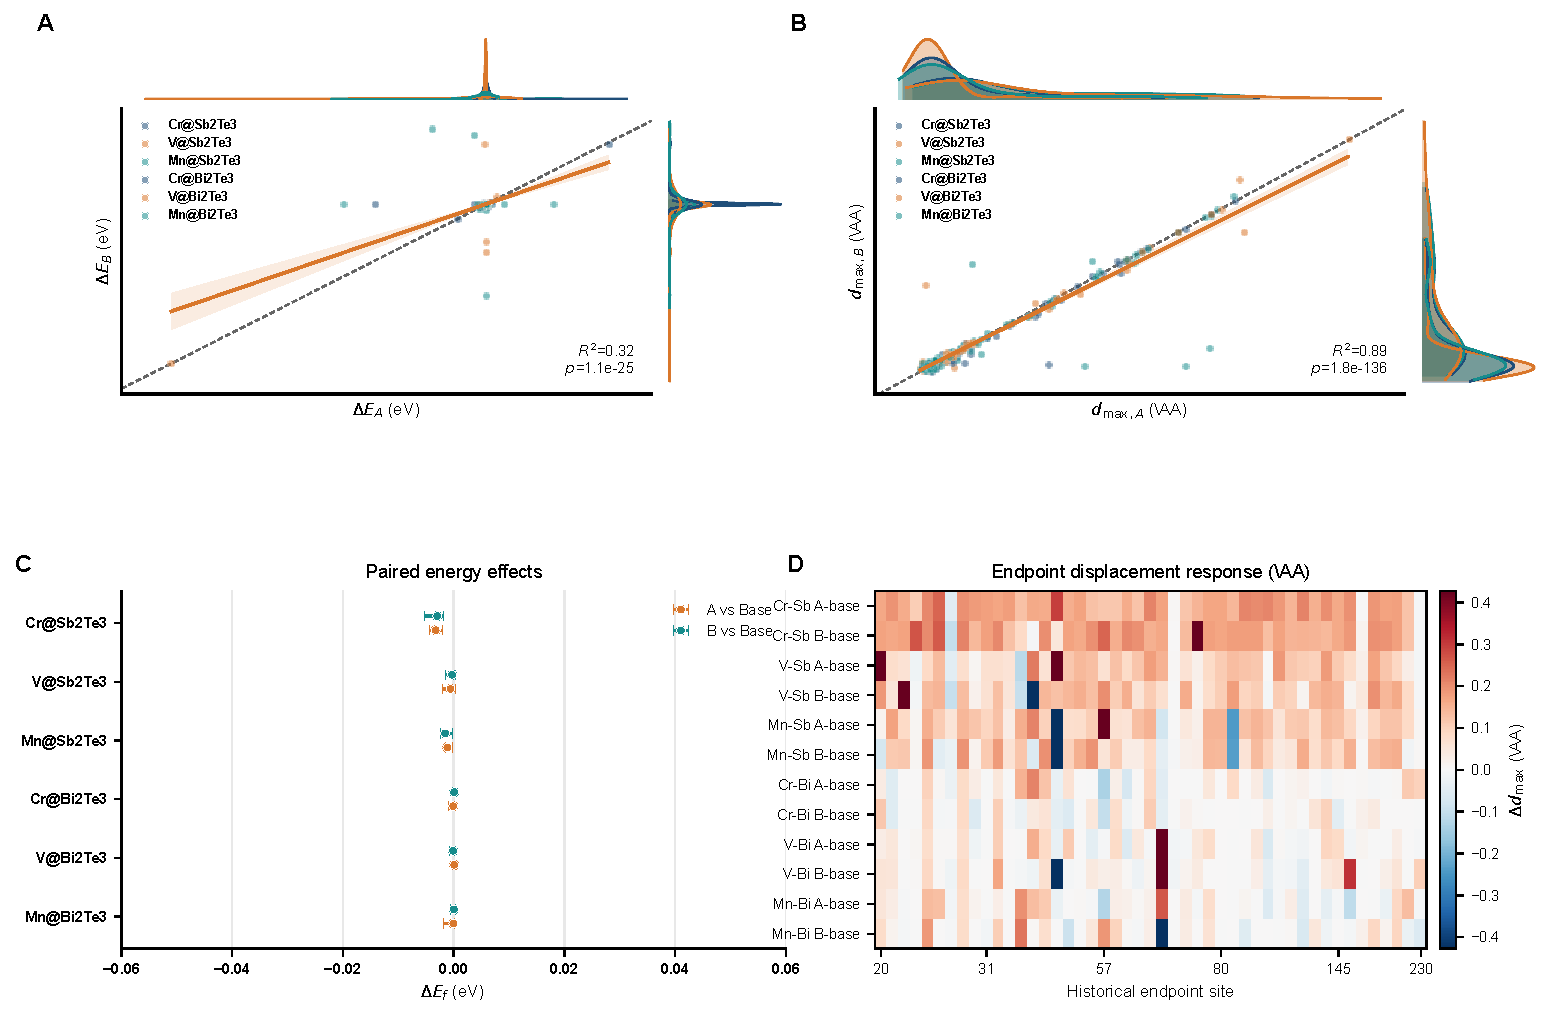
\includegraphics[width=\textwidth]{revision1/appendix/figures/fig2_perturbation_response.pdf}
\caption{\textbf{Perturbation response across systems and endpoints.} Joint
distributions compare the energy and geometric response of Perturb A and B.
Forest intervals summarize arm-specific changes relative to Base, and the
endpoint heatmap exposes the site-level structure hidden by aggregate medians.
Intervals are bootstrap summaries of the observed endpoint sample and should
not be interpreted as uncertainty in the MACE potential itself.}
\label{fig:endpoint_perturbation_response}
\end{figure}

\begin{figure}[p]
\centering
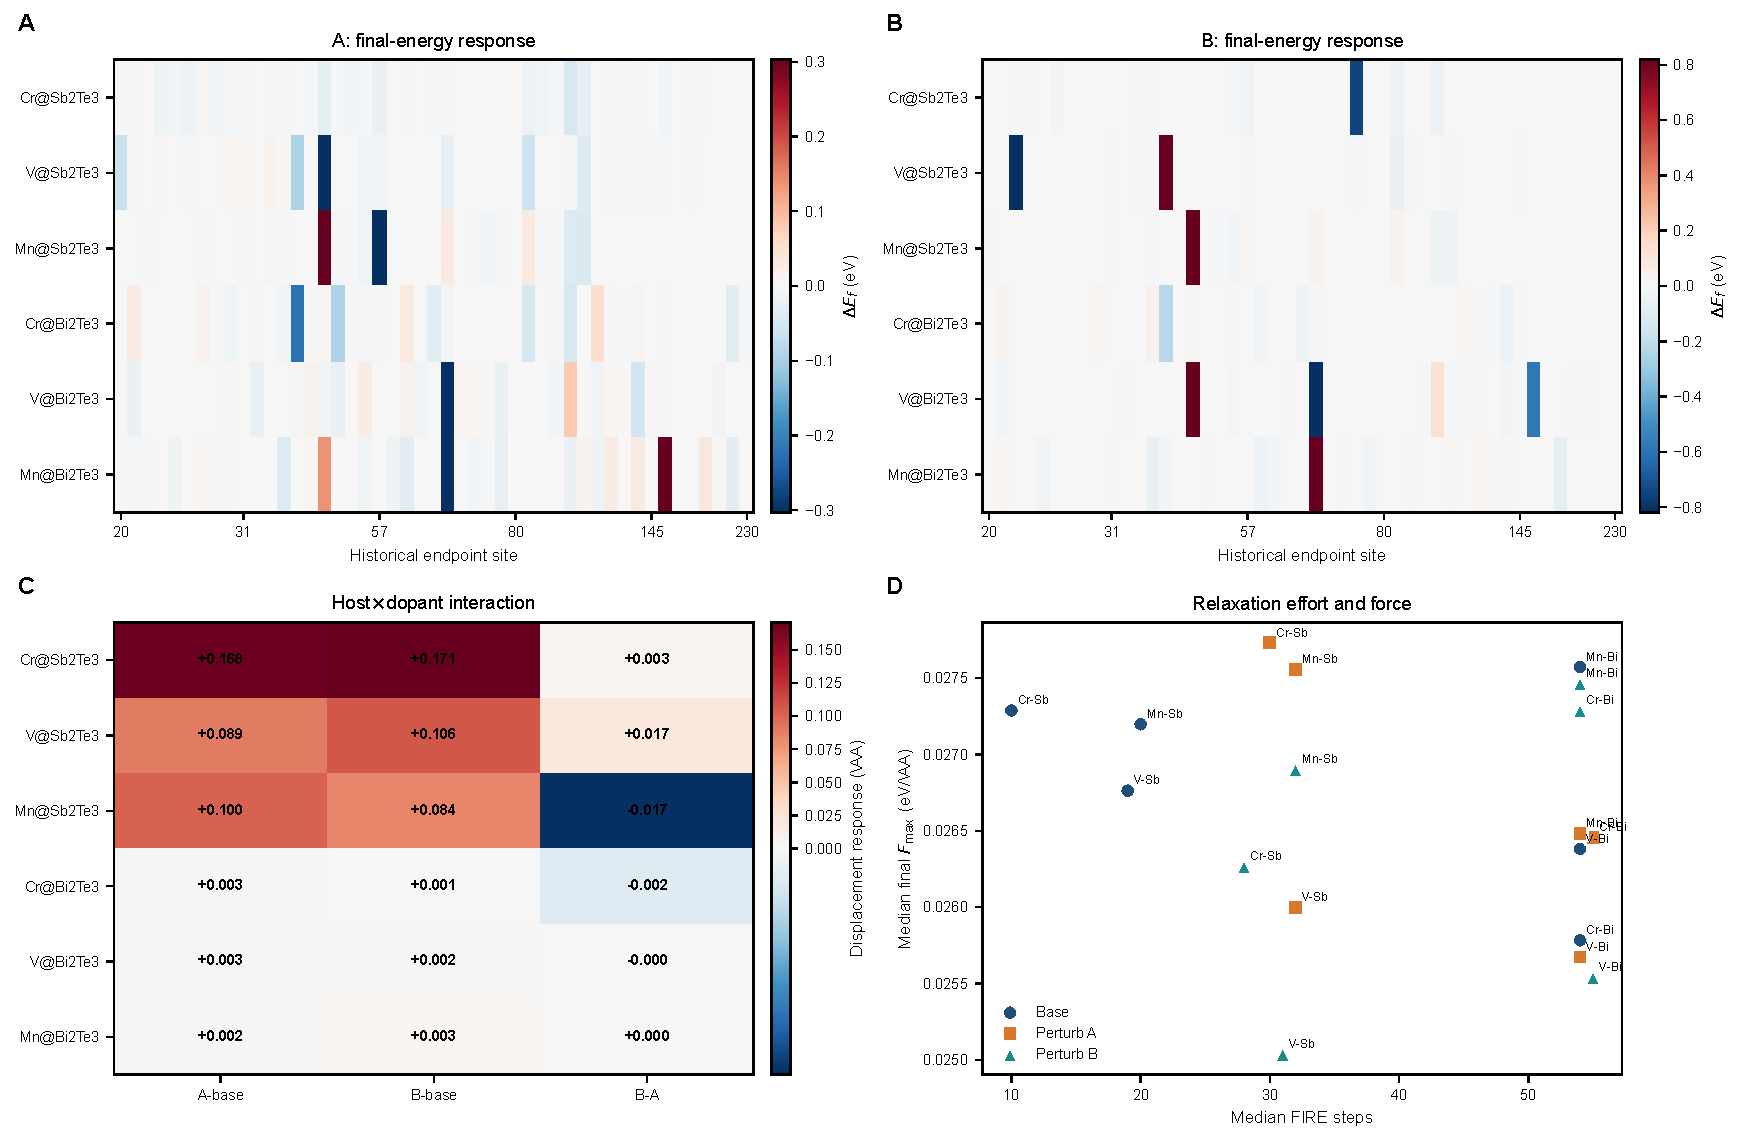
\includegraphics[width=\textwidth]{revision1/appendix/figures/fig3_interaction_and_site_maps.pdf}
\caption{\textbf{Host--dopant interactions and relaxation effort.} Endpoint
heatmaps show energy response for each host--dopant system, while the interaction
map compares the two perturbation arms. The effort panel relates initial force
to the number of FIRE steps required by the fixed-cell relaxation protocol.}
\label{fig:endpoint_interaction_maps}
\end{figure}

\subsection{Interpretation and reproducibility}

The complete endpoint-level data used for these figures are provided in
\texttt{revision1/appendix/data/endpoint\_level\_summary.csv} and its JSON
counterpart.  The summary table is generated from
\texttt{revision1/appendix/data/multiarms\_summary.csv}.  The plotting source
is preserved as
\texttt{revision1/appendix/scripts/plot\_campaign\_atlas.py}; it uses the
project Plot Atlas primitives and regenerates the three PDF, PNG, and SVG
figures from the supplied data.  Overleaf compiles the checked-in PDF assets;
the data and script are included alongside them so that the figures remain
auditable and reproducible outside the hosted compiler.

The dominant qualitative result is that all three arms are scientifically
accepted, while perturbation magnitude and response depend strongly on both
host and dopant.  In particular, the \ce{Bi2Te3} systems exhibit larger
endpoint displacements than the corresponding \ce{Sb2Te3} systems, whereas
the final force distributions remain tightly concentrated near the FIRE
acceptance threshold.  These patterns support using endpoint perturbations as
a controlled local-stability probe, but do not establish transferability to
DFT energetics or to finite-temperature migration barriers.
